\section{Introduction}

In this paper we present \dReach{}, a bounded $\delta$-reachability
analysis tool for nonlinear hybrid systems. Given $\delta$, a positive
rational number, $\delta$-reachability analysis decides whether there
exists a path from an initial-state to an unsafe-state if we
syntactically perturb a given hybrid system and safety condition.
Compared to the undecidable results~\cite{?} of the general
reachability problem, our previous
work~\cite{DBLP:journals/corr/GaoKCC14} proved that this new
formulation is not just decidable but also has tractable complexity
(i.e. $\np^{\mathsf{C}}$ for an invariant-free $H$).

\begin{figure}
  \centering
  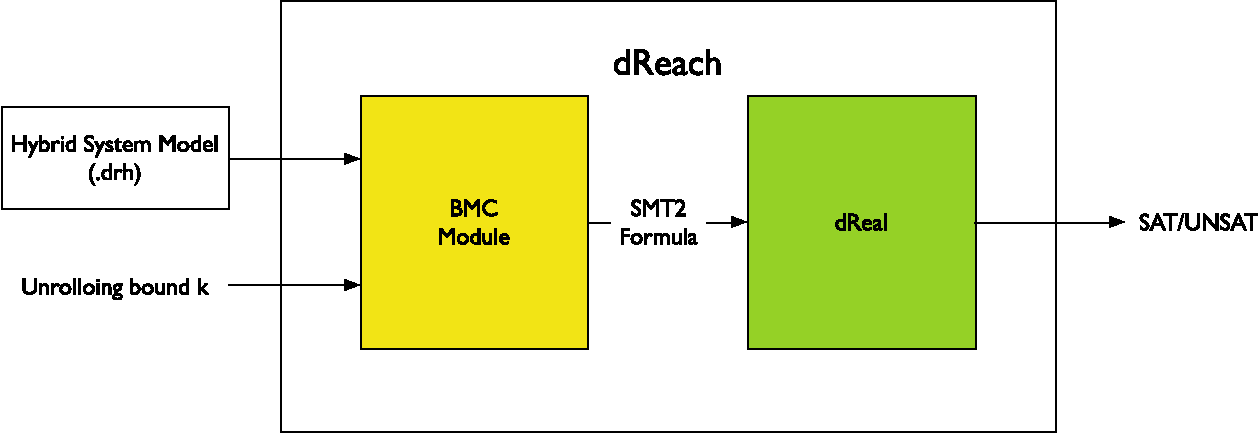
\includegraphics[width=\textwidth]{images/dReach}
  \caption{System Description of \dReach{}}
  \label{fig:system-description}
\end{figure}

Figure~\ref{fig:system-description} illustrates the design of
\dReach{}. We provide a domain-specific lanaguage to describe a hybrid
system and specify its safety properties. Given an input model,
specification, and unrolling bound $k$, \dReach{} reduces the
$\delta$-reachability problem to a $\delta$-decision problem of
formulas over the reals by providing a corresponding SMT encoding for
the problem. Then we use our nonlinear SMT solver
\dReal{}~\cite{DBLP:conf/cade/GaoKC13} to solve the translated problems.






% Where do we use this?
% CMSB'14

% FMCAC'13
% CADE'13




%%% Local Variables:
%%% mode: latex
%%% TeX-master: "main"
%%% End:
